\chapter{Descripción del Trabajo}
\label{cap:descripcionTrabajo}

%En este capítulo abordaremos los aspectos tanto de diseño como de implementación de nuestra aplicación...TO BE CONTINUED

\section{Reunión en el Centro de Tiflotecnología e Innovación de la ONCE}

La idea de este TFG surgió de la necesidad de resolver problemas reales para gente real, concretamente para personas con discapacidad visual. Por ello, como no podía ser de otra manera, comenzamos nuestro camino por lo más importante: conocer las necesidades de los usuarios finales. Con este fin y gracias a la oportunidad que nos  brindó la Universidad Complutense de Madrid con la profesora María Guijarro al frente, pudimos reunirnos y entrevistar a personas especializadas en el campo de las tecnologías que sufren discapacidad visual.

En este documento recogemos las notas que tomamos durante la reunión el día 11 de octubre de 2019 en el CTI (Centro de Tiflotecnología e Innovación) de la ONCE.
	

%PRIMERA SECCIÓN
\subsection{Introducción}
La entrevista comenzó con una breve explicación, de la mano de José María Ortiz, director del Departamento de Consultoría e Innovación, sobre las principales tareas que se llevan a cabo en el centro, entre las cuales destacan:

\begin{itemize}
	\item Ayudar a una persona con discapacidad visual en su \textbf{adaptación} al trabajo y a la vida cotidiana, proporcionandole para ello el material necesario (teclados, líneas de braille, bastones, etc.).
	\item Responder a \textbf{consultas} sobre el funcionamiento de dispositivos.
\end{itemize}

Luego, nos comentó los departamentos en los que se estructura el centro para que pudiésemos hacernos una idea más global de todo lo que abarca. Éstos son:

\begin{itemize}
	\item \textbf{El departamento de Consultoría e Innovación:} donde actualmente están desarrollando el programa EDICO en colaboración con la UCM, que tiene como objetivo hacer las matemáticas accesibles mediante un editor de texto. De manera paralela se encargan del desarrollo de aplicaciones de muy diversa índole, véase apps para la biblioteca de la ONCE, de películas audio-descritas, etc.
	\item \textbf{Departamento de Evaluaciones y Auditoría:} donde se encargan de evaluar los productos que se van a sacar al mercado.
	\item \textbf{Departamento de diseño y producción:} donde se encargan de, tal y como indica su nombre, diseñar y producir elementos de adaptabilidad, como pueden ser unas plantillas con relieve de policarbonato para las vitrocerámicas. Recordemos que estas, aunque no presentan dificultad alguna para los usuarios videntes, son tediosas para aquellos que cuentan con discapacidad visual ya que la pantalla táctil no tienen ningún tipo de relieve que pueda servirles como referencia y guiarles en su uso.
	\item \textbf{Departamento de Asesoría en tecnología:} especializado en tecnologías accesibles.
\end{itemize}

Una vez concluida esta sección en la que nos contextualizaron, abrieron paso a la ronda de preguntas en la que pudimos acercarnos a ellos, conociendo sus problemas y necesidades en el día a día.

%SEGUNDA SECCIÓN
\subsection{Entrevista}

Durante esta parte, nos dirigimos especialmente a Mónica y José Luis Llorente, ambos ingenieros del CTI, para que, con su experiencia y conocimientos, nos explicaran lo máximo posible sobre tecnologías accesibles y nos dieran su punto de vista en las ideas que proponíamos. Por otro lado, Mónica no solo era experta en la materia sino que además era invidente, por lo que nos pudo contar su perspectiva y necesidades como usuaria.

Las preguntas avanzaron desde temas generales para conocer cómo una persona invidente se desenvuelve con la tecnología, sus gustos y qué sensaciones le despierta, hasta temas concretos dirigidos a conocer los problemas que plantea la navegación por espacios interiores.

\begin{itemize}
	\item  \textbf{¿Cómo utiliza una persona con discapacidad visual un dispositivo móvil?}
	
	Para responder a esta pregunta, Mónica nos hace una demostración en directo, para ello emplea un móvil Xiaomi con sistema operativo Android.
	
	Mónica nos cuenta que para la navegación por su dispositivo utiliza un lector de pantalla, es decir, un software que facilita el uso del sistema operativo. Éste sirve como guía para las personas que, como ella, tienen discapacidad visual, ya que ``lee y explica'' mediante voz lo que se ve en la pantalla. Los lectores de pantalla vienen siempre incluidos en el dispositivo y se pueden encontrar en la sección de Accesibilidad, en Ajustes. En el caso de Android, este software se llama \textit{Talkback} y es configurable. Por ejemplo, dice Mónica, se podría usar mediante la línea de braille en vez de la reproducción por voz.
	
	Luego vemos como se desplaza por las aplicaciones utilizando \textit{flicks}, movimientos secos en los que desliza el dedo hacia uno de los lados de la pantalla (izquierda o derecha, según interese). Del mismo modo, para la navegación por la web o dentro de alguna aplicación utiliza estos movimientos hacia arriba y hacia abajo. Por último, nos muestra cómo accede a un elemento mediante doble click. 

	También nos habla de la posibilidad de la navegación libre, eso sí, solo cuando ya te has familiarizado con el dispositivo lo suficiente como para saber dónde tienes determinadas aplicaciones. 

	Lo más cansado, según Mónica, es tener que hacer un barrido por toda la pantalla hasta encontrar lo que quieres, en vez de poder ir directamente. Para agilizar un poco este proceso, Mónica, por ejemplo, agrupa las aplicaciones por carpetas, de modo que el barrido es más sencillo que si la pantalla estuviese repleta.
	
	Para las personas con baja visión también existe la posibilidad de hacer más grandes los iconos y ajustar los colores.
	
	% Segunda pregunta:
	\item \textbf{Hemos leído que normalmente las aplicaciones se desarrollan para dispositivos iOS, ¿por qué es mejor?} 
	
	\textit{``Si que es cierto que solía ser así ya que iOS le llevaba la delantera a Android en cuanto a accesibilidad, pero cada vez se usa más Android pues las diferencias están completamente recortadas, están muy igualados y los precios son mucho más asequibles. Yo misma, antes tenía un iPhone y ahora me he pasado a Android y no hay nada que eche en falta.''}, responde Mónica.
	
	% Tercera pregunta:
	\item \textbf{¿Cómo afronta una persona ciega su desplazamiento y orientación por interiores cuando pisa por primera vez dicho espacio u edificio?}
	
	Ante esta pregunta Mónica resopla y nos contesta: \textit{``Buufff..., ¿te vale?''}
	
	Nos puso como ejemplo la llegada a un hospital: \textit{``cuando entras necesitas saber, al menos, dónde está la recepción para pedir ayuda pero los carteles informativos están fuera de mi alcance, entonces entro por la puerta y pienso ¿y ahora qué?. ¿Dónde está el mostrador de recepción? No es tan fácil como echar un primer vistazo, necesitas ayuda mediante voz, algo que te describa el espacio y te vaya diciendo que hay a derecha e izquierda y a cuantos metros.''}

	Nos contó que en cuanto a la descripción/guía por espacios interiores ahora mismo no hay disponible ninguna aplicación. Por ello, una vez superada la primera barrera de ubicar y localizar un cierto destino, la única opción que les queda es la de memorizar el camino. Mónica destacó que era increíble la cantidad de rutas que tiene en la cabeza.
	
	Por todo esto, se comentó que una aplicación sería de gran ayuda para ellos, de manera que pudiesen tener una idea del edificio incluso antes de llegar a él para moverse con más seguridad. Una app que no solo les guiase a un punto concreto, sino que además describiese el edificio, indicándoles qué posibilidades les ofrece. También se mencionaron otras propuestas e ideas como tener previamente el plano del edificio para poder ir moviéndote con el dedo sobre él y que a su paso te vaya indicando las distintas salas que aparecen, o la impresión de un mapa 3D que disponga de un código QR o algo similar que fuese capturado mejor por Bluetooth que por foto que tras leerlo cargase el plano del edificio y pudiese proporcionar tanto información sobre el espacio en sí mismo (número de plantas, qué hay en cada una...) como información más precisa como puede ser averías, horarios, disponibilidad de salas, etc.
	 
	Obviamente de la mano de estas ideas surgían problemas y opiniones en contra: ¿Dónde estaría dicho mapa?, ¿Cómo encontrarlo?, ¿Todos los edificios estarán de acuerdo en facilitar los planos o puede que por motivos de seguridad no sea una idea factible?, ¿es posible llegar a un standard para que se pueda usar el mismo sistema en cualquier edificio?
	
	% Cuarta pregunta:
	\item \textbf{¿Hay algún tipo de señales que os sirvan como referencia a la hora de desplazaros por un edificio?}
	
	\textit{``Hay señales de encaminamiento, que te indican dónde están las escaleras, ascensores, zonas de cruce, etc.''}, contesta.

	% Quinta pregunta:
	\item \textbf{¿Cuántos edificios cuentan con estas señales?}
	
	\textit{``La verdad que cada vez son más frecuentes y hoy en día se encuentran en casi todos los edificios, especialmente en los nuevos.''}, responde.
	
	% Sexta pregunta:
	\item \textbf{¿Cómo de factible es ir con el dispositivo móvil en la mano, para realizar una foto o cualquier cosa similar?}
	
	\textit{``Puedo hacer una foto en un momento puntual, en eso no hay problema alguno pero no es cómodo ir con el móvil en la mano constantemente porque además de que es aparatoso porque ya llevo en la mano el bastón, perro guía, etc. No es práctico, no sería la primera vez que roban un móvil a una persona invidente, es una realidad.''}, contesta Mónica. \textit{``Particularmente, con respecto a la foto el problema principal sería saber a dónde enforcar''}, añade.
	
\end{itemize}

%Creo que es mejor subsection para las conclusiones del TIC
%TERCERA SECCIÓN
\subsection{Conclusiones}
Tras el debate, algunas de las conclusiones que sacamos de la visita al CTI son:

\begin{itemize}
	\item La implementación de una aplicación como la nuestra es muy útil y necesaria.
	\item Las modalidades más empleadas para interactuar con el móvil cuando tienes algún tipo de rastro visual son: flicks, sacudidas, mediante vibración, arrastrando o pulsando la pantalla con un dedo, dos,...
	\item No resulta cómodo ir barriendo el espacio con la cámara del móvil.
	\item El uso de dispositivos adicionales como una micro cámara, en principio, no sería un problema, siempre y cuando no la tengan que llevar de manera continuada en la mano.
	\item En caso de auriculares, se recomienda utilizar auriculares óseos de modo que dejen el canal auditivo libre para captar otros estímulos.
	\item El objetivo es que el grueso de las aplicaciones sean lo más inclusivas posibles, es decir, que su uso sea apto tanto para personas videntes como invidentes.
	\item El feedback de la aplicación no debe saturar pero sí se aconseja que sea constante para que no se malinterprete que la aplicación ha dejado de funcionar.
\end{itemize}


\section{Estudio de precisión de los beacons}

Antes de ponernos manos a la obra con la aplicación debíamos conocer cómo se comportaban los beacons en cuanto a distancias. Ya conocíamos que esta tecnología era una de las más usadas para el posicionamiento en interiores pero necesitábamos saber los aspectos más tecnológicos: cuánto rango tenía la señal \textit{bluetooth} de estos aparatos, si la intensidad de esta señal era suficiente para poder determinar a qué distancia estaban y, lo más importante, cómo afectaba a todo ello el espacio en el que se iban a colocar; el pasillo, una esquina, una puerta, etc. Puesto que las investigaciones que habíamos realizado ya avisaban de que la intensidad de los beacons era muy dependiente del lugar y el material sobre el que estos se colocaran. REFERENCIA AL PDF DE WAYFNDER.

Para comenzar esta investigación nos ayudamos en la propia SDK de \textit{Kontakt}, la marca de nuestros beacons. Esta permite conocer qué beacons están en nuestro rango en un momento determinado y actualizar esa lectura cada cierto tiempo. Además tiene implementado un sistema de categorías en función de cómo de cerca o lejos esté un cierto dispositivo. Las categorías son las siguientes:

\begin{itemize}
	\item IMMEDIATE: Si el dispositivo se encuentra a menos de 0,5m.
	\item NEAR: Si el dispositivo se encuentra entre los 0,5m y los 3m.
	\item FAR: Si el dispositivo se encuentra a más de 3m.
	\item UNKNOWN: Si se ha perdido la señal del dispositivo.
\end{itemize}

Gracias a estas funciones ya implementadas en la SDK desarrollamos en poco tiempo pequeñas y simples aplicaciones que nos permitieron de manera muy visual comprobar las medidas leídas con las medidas reales a las que estaban los beacons. Estas medidas se realizaron tanto en la propia Facultad de Informática como en nuestras propias casas.

A continuación presentamos las herramientas desarrolladas para medir la fiabilidad y exactitud de nuestros beacons.

\subsection{Aplicación miniapp}
Esta aplicación fue la primera toma de contacto con los beacons, queríamos una aplicación visual que nos indicara la categoría de proximidad de los beacons. El tomar la categoría como aproximación de la distancia fue nuestra primera idea, puesto que teníamos en mente que la señal de los beacons no era muy estable. En la Figura \ref{fig:miniapp} vemos la interfaz principal de la aplicación, con ella podíamos medir la categoría de hasta tres beacons. Los beacons considerados se encuentran debajo del panel de categorías y la categoría en la que se encuentran se resalta en verde. La lectura que se hace de los beacons se va actualizando cada $x$ tiempo establecido. 

La idea de esta aplicación fue la de establecer el grado de confianza que podíamos tener en las categorías ofrecidas por la SDK de \textit{Kontakt}. El resultado fue muy positivo puesto que, a pesar de que las distancias fluctuaban, la categoría se asignaba correctamente sin grandes fluctuaciones. 

\begin{figure}[t]
	\centering
	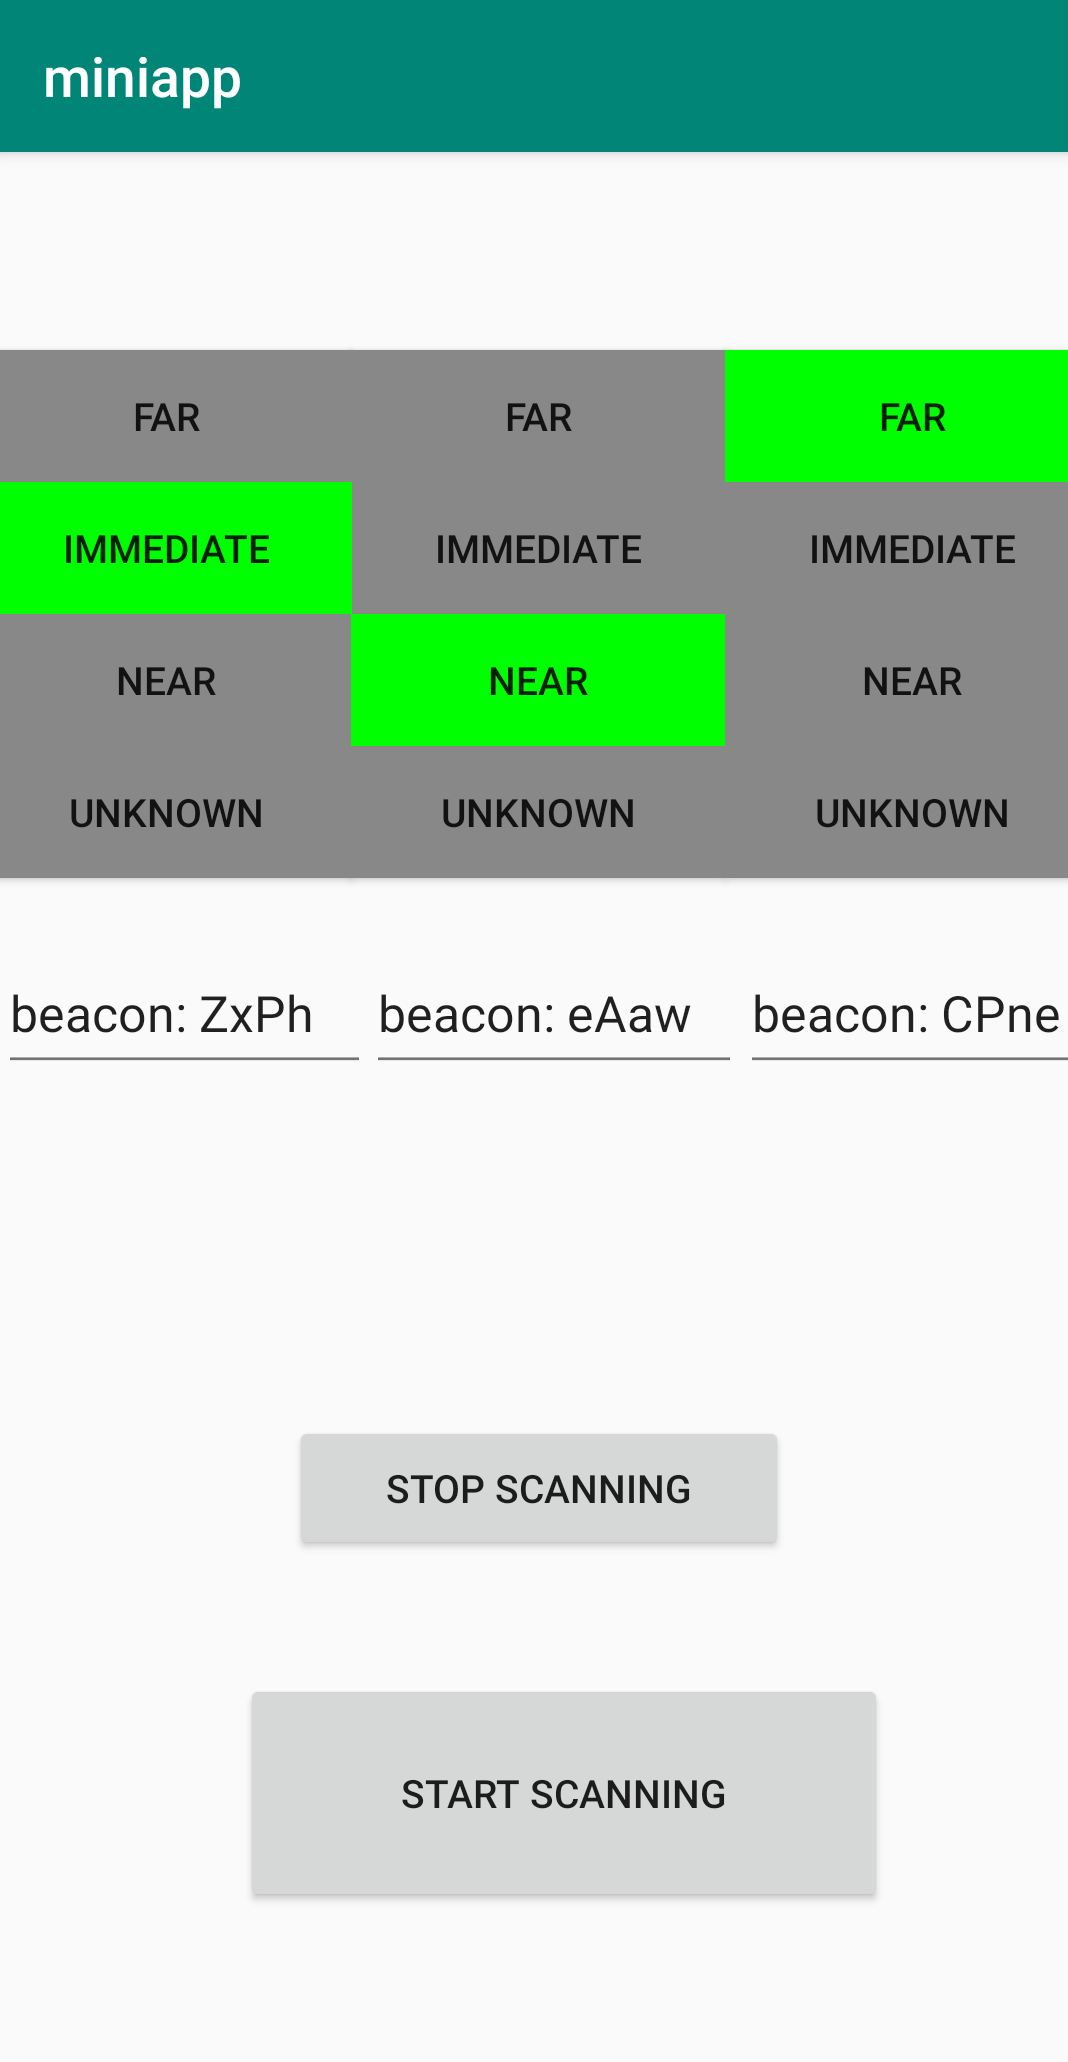
\includegraphics[width=0.4\textwidth]{Imagenes/Descripciondeltrabajo/miniapp}
	\caption{Interfaz de la aplicación miniapp. }
	\label{fig:miniapp}
\end{figure}

\subsection{Aplicación cuadrantes v1}
En la Figura \ref{fig:cuadrantesv1} vemos la interfaz principal de la aplicación \textit{cuadrantes v1}, esta fue diseñada, en inicio, para saber a qué distancia debían estar los beacons y poder así dividir las distintas plantas de la facultad en cuadrantes (de ahí su nombre), de esta manera podríamos construir un grafo cuyos nodos fueran estos cuadrantes y, que representara el mapa de la facultad.

Es una aplicación muy sencilla, cuya función es recoger cada cierto tiempo, en la figura lo hace cada dos segundos, la señal de los beacons que están a su alcance, mostrar la categoría de su distancia y la distancia estimada en metros. La razón por la que llevamos un registro de qué está en el rango cada cierto tiempo es que notamos que las distancias fluctuaban, notoriamente en algunos casos, y quisimos hacer un estudio previo al desarrollo de la aplicación.

\begin{figure}[t]
	\centering
	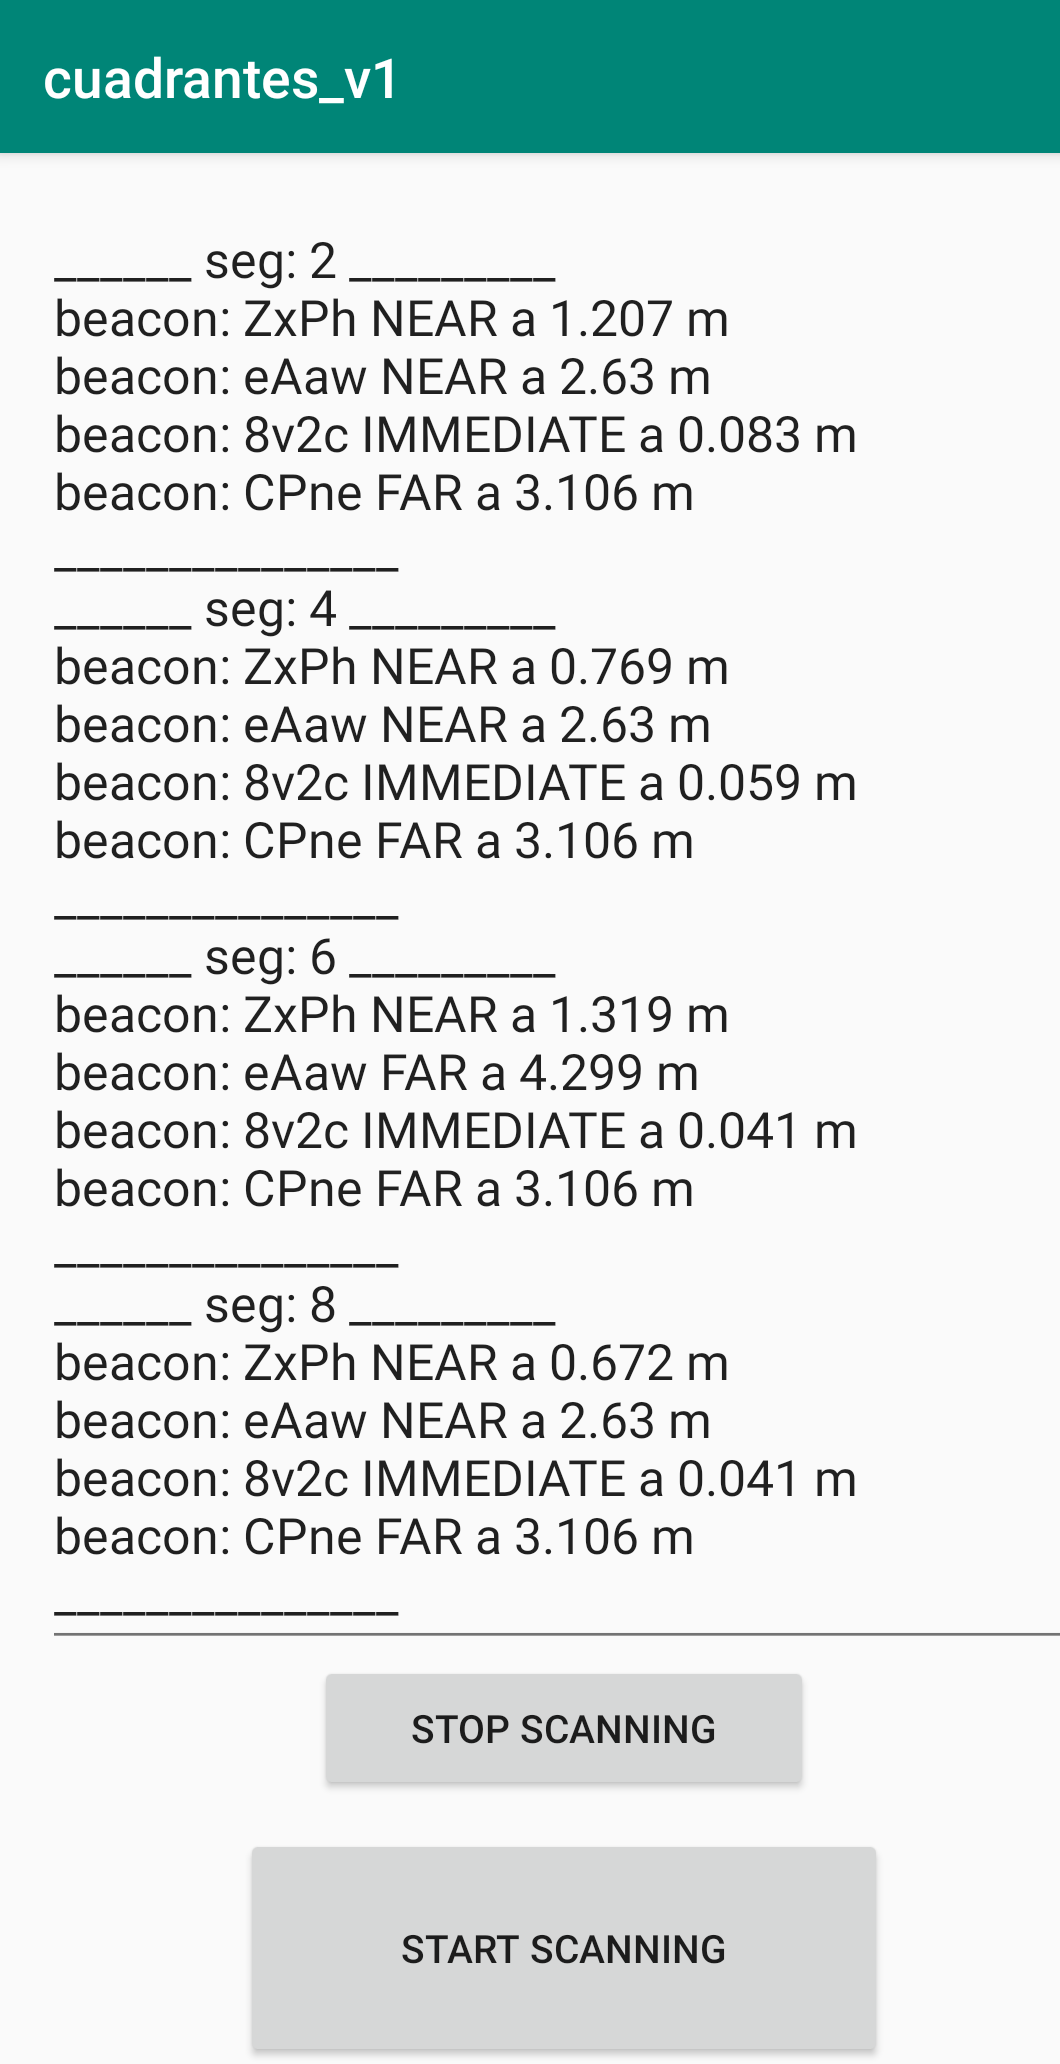
\includegraphics[width=0.4\textwidth]{Imagenes/Descripciondeltrabajo/cuadrantes_v1}
	\caption{Interfaz de la aplicación cuadrantes v1.}
	\label{fig:cuadrantesv1}
\end{figure}


\subsection{Resultados}

A continuación presentamos los resultados de las distintas mediciones realizadas. Veamos primero  aquellas recogidas en gráficas: en ellas podemos ver cómo se comportan los beacons si comparamos la medida real con la estimada por la aplicación. 

En la Figura \ref{fig:dist_CPne} vemos las lecturas que nos ha dado la aplicación \textit{cuadrantes v1} cuando hemos leído las distancias del beacon con identificador CPne. Las diferentes lecturas corresponden a las medidas estimadas cuando el beacon estaba a dos metros (azul), alrededor de dos metros y medio (naranja), cinco metros (gris) y a sesenta y cuatro centímetros (amarillo).

De esta gráfica destacamos que a grandes distancias, en este caso cinco metros, la medida estimada comienza a no ser muy fiable, a la par que muy fluctuante. Sin embargo, podemos ver cómo la medida a dos metros de distancia es la bastante exacta, fluctúa en menos de un metro a lo largo de casi toda la medición. Por último, la medición a menos de un metro, que se corresponde con la línea amarilla presenta fluctuaciones muy pequeñas, poco relevantes para nuestra aplicación. Como conclusión sacamos que cuanto mayor es la distancia a la que está el beacon menor es la fiabilidad  que podemos depositar en la estimación de la medida obtenida. 

\begin{figure}[t]
	\centering
	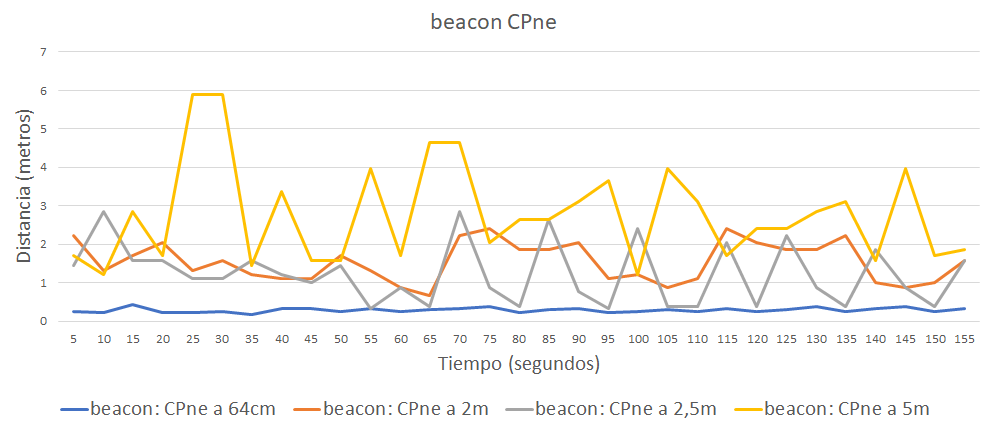
\includegraphics[width=0.7\textwidth]{Imagenes/Descripciondeltrabajo/dist_CPne}
	\caption{Gráfico con las distancias medidas al beacon CPne. }
	\label{fig:dist_CPne}
\end{figure}

En el caso de la Figura \ref{fig:dist_eAaw} el comportamiento es similiar, a pesar de que tenemos un par de picos importantes en los primeros segundos de medición, el valor medio que obtenemos es el de una distancia estimada de un metro para un beacon que realmente está situado a medio metro. La Figura \ref{fig:dist_8v2c} recoge tres mediciones distintas para una misma distancia, cada una de ellas recoge unos valores distintos y bastante bajos, lejos de los aproximadamente 4 metros reales. Una posible explicación a este fenómeno nos lo puede dar la Figura \ref{fig:dist_conjunto}, que recoge la medición de dos beacons situados a la misma distancia y uno encima del otro. Como vemos, la medición del beacon situado abajo es bastante más baja, en comparación. Esto nos advierte de que la señal \textit{bluetooth} es bastante dependiente de los obstáculos, el entorno, ¡hasta las condiciones meteorológicas!. 


\begin{figure}[t]
	\centering
	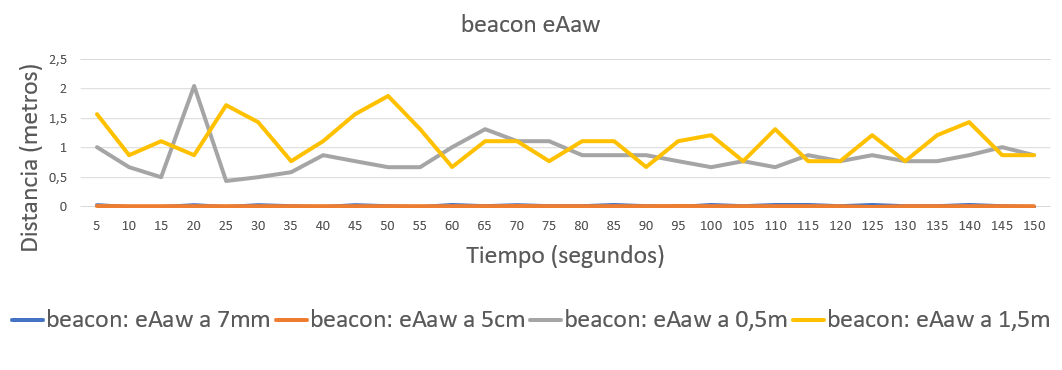
\includegraphics[width=0.7\textwidth]{Imagenes/Descripciondeltrabajo/dist_eAaw}
	\caption{Gráfico con las distancias medidas al beacon eAaw. }
	\label{fig:dist_eAaw}
\end{figure}


\begin{figure}[t]
	\centering
	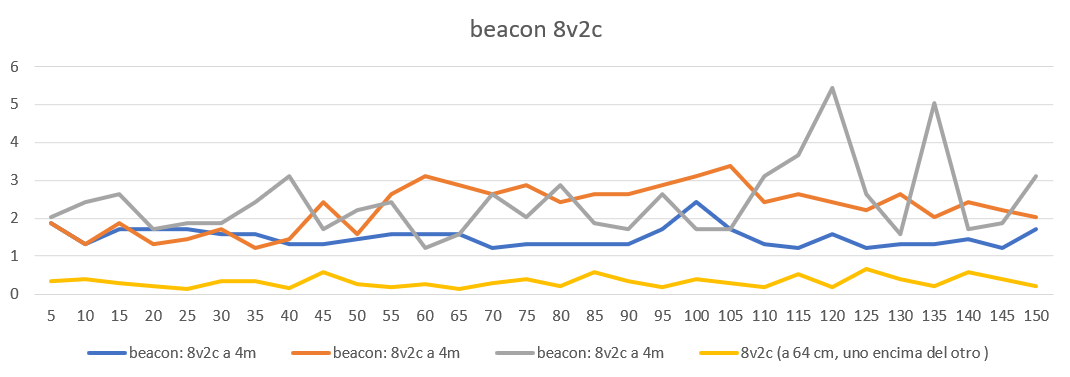
\includegraphics[width=0.7\textwidth]{Imagenes/Descripciondeltrabajo/dist_8v2c}
	\caption{Gráfico con las distancias medidas al beacon 8v2c. }
	\label{fig:dist_8v2c}
\end{figure}

\begin{figure}[t]
	\centering
	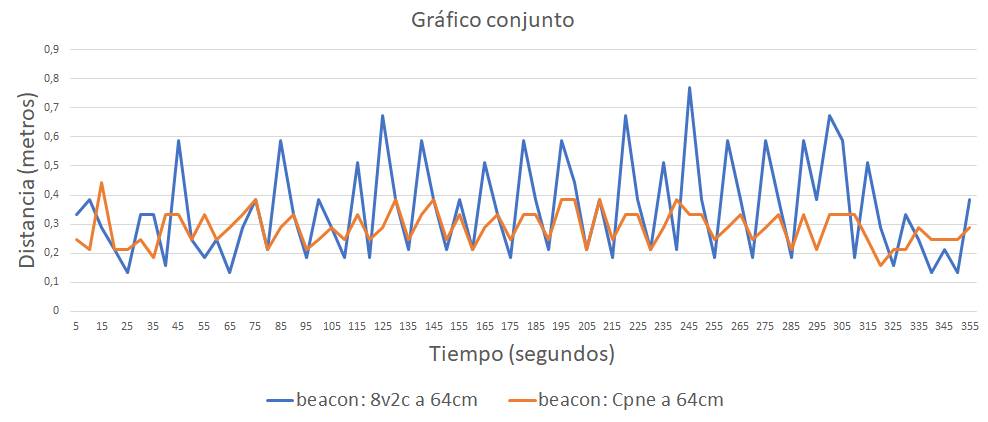
\includegraphics[width=0.7\textwidth]{Imagenes/Descripciondeltrabajo/dist_conjunto}
	\caption{Gráfico con las distancias medidas conjuntas de los beacons 8v2c y CPne, estando uno sobre otro. }
	\label{fig:dist_conjunto}
\end{figure}


\subsection{Mediciones en puntos clave de la facultad}

Una vez que tuvimos una idea más clara del funcionamiento y el comportamiento de los beacons fue hora de abordar el problema desde el punto de vista del posicionamiento. La idea inicial fue la de colocar beacons en puntos clave, de tal manera que al encontrarnos con uno de ellos nos avisara de una intersección, un aula o cualquier otro destino o punto de interés. 

En este caso los beacons tenían una posición muy concreta y los puntos desde los que se medía también. En la Figura \ref{fig:medidasPBaja} se puede ver en qué puntos se colocaron los beacons (punto rojo) y en qué puntos se midieron las distancias (cruz verde). Lo primordial era conocer la ubicación óptima de los beacons en los lugares más complicados, como son las intersecciones, los puntos donde se acumulan varios lugares de interés (como puede ser el caso de la puerta de entrada, delegación de alumnos y el aula cinco), así como aquellos espacios más grandes (como el \textit{hall} de entrada). En el ANEXO se pueden ver los resultados de estas mediciones. A continuación exponemos las conclusiones recogidas:

\begin{itemize}
	\item Los beacons no deben situarse demasiado cerca, esto altera las mediciones y hace que no sepamos distinguir cuál es el beacon más cercano. 
	\item En lugares diáfanos, como el \textit{hall}, la señal de los beacons fluye con mayor libertad. Es por ello que podemos situarlos a mayor distancia sin que queden puntos ciegos en lugares importantes. Uno de los inconvenientes de esto surgió a la hora de introducir un beacon en la puerta del salón de actos 
\end{itemize}

\begin{figure}[t]

	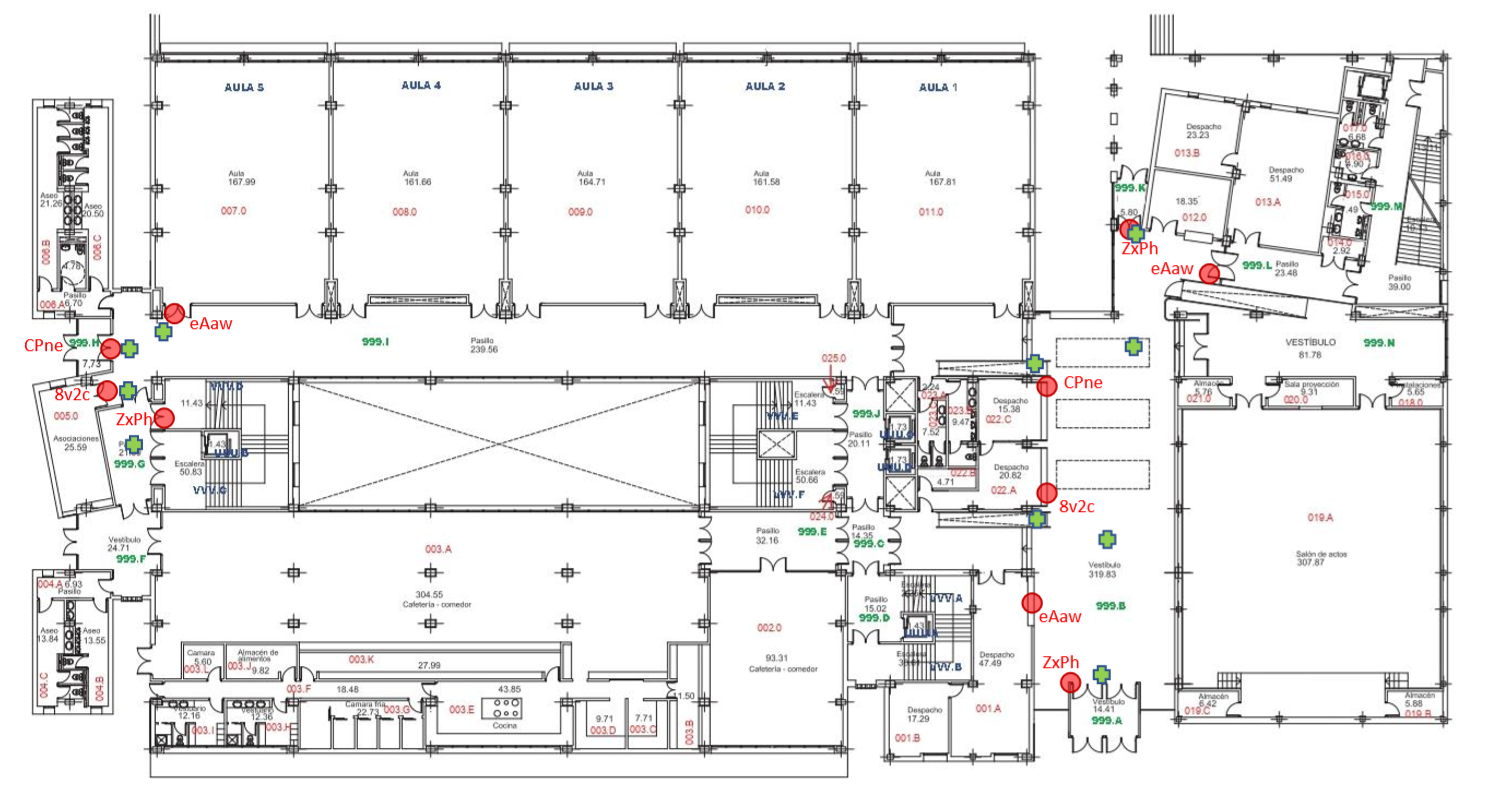
\includegraphics[width=1\textwidth]{Imagenes/Descripciondeltrabajo/medidasPlanoPBaja}
	\caption{Mapa de la planta baja de la Facultad de Informática con la ubicación de los beacons (rojo) y los puntos de medición (verde). }
	\label{fig:medidasPBaja}
\end{figure}
